\section{Design}

\subsection{Architectural sketch}

Below is the architectural sketch of the components structured in the diagram that
highlights the software and hardware components.

\begin{figure}[h]
    \centering
    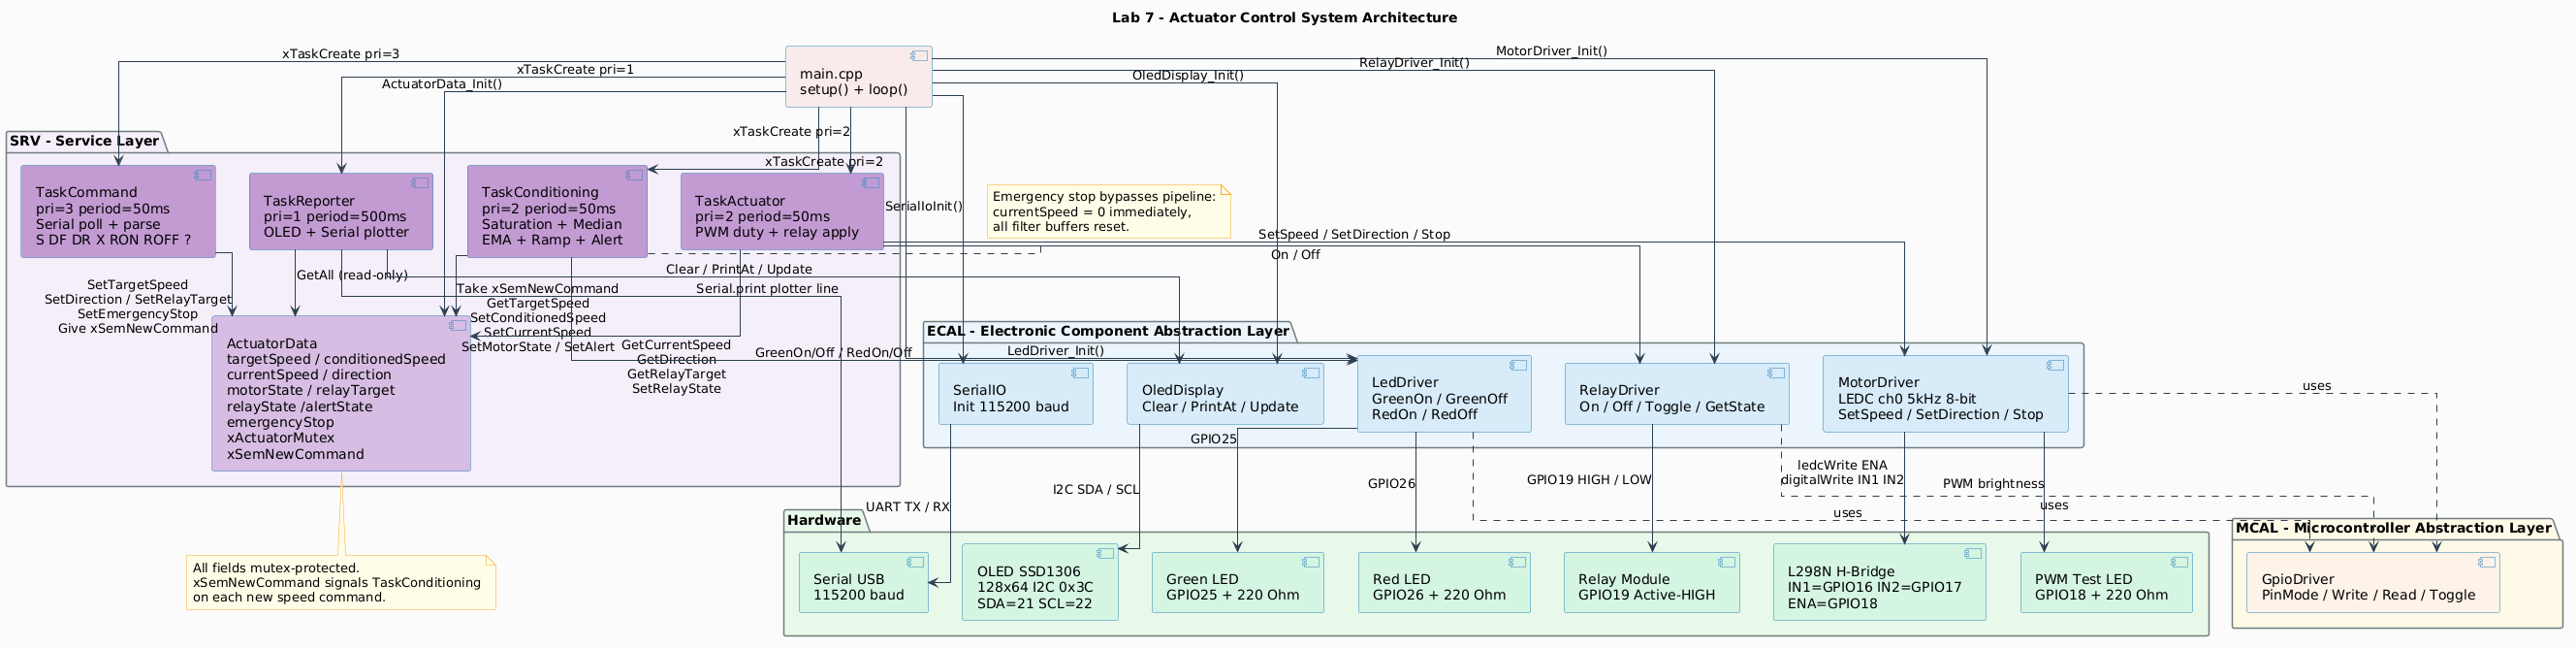
\includegraphics[width=1\textwidth]{./img/architecturediagram.png}
    \caption{Architectural sketch of the project}
    \label{fig:archi}
\end{figure}

This is the description of each of the elements of the diagram:
\begin{enumerate}
  \item \textbf{ESP32 DevKit microcontroller} -- central processing unit running FreeRTOS
    and executing all four application tasks preemptively
  \item \textbf{L298N motor driver (IN1=GPIO\,16, IN2=GPIO\,17, ENA=GPIO\,18)} --
    H-bridge driver controlled by TaskActuator; direction set via IN1/IN2, PWM speed
    via ENA using LEDC (channel~0, 5\,kHz, 8-bit); LED on ENA simulates motor during
    testing
  \item \textbf{Relay module (GPIO\,19)} -- active-HIGH single-channel relay controlled
    by TaskActuator; state transitions tracked in ActuatorData
  \item \textbf{Green LED (GPIO\,25)} -- ON when no alert is active
  \item \textbf{Red LED (GPIO\,26)} -- ON when OVERLOAD or LIMIT\_REACHED alert is active
  \item \textbf{OLED 128$\times$64 SSD1306 (SDA=21, SCL=22, addr 0x3C)} -- primary
    display updated by TaskReporter every 500\,ms showing motor state, direction,
    target/conditioned/current speed, relay state, and alert
  \item \textbf{ActuatorData module} -- shared data store protected by
    \texttt{xActuatorMutex}; holds targetSpeed, conditionedSpeed, currentSpeed,
    direction, motorState, relayTarget, relayState, alertState, emergencyStop flag,
    and all configurable pipeline parameters
  \item \textbf{TaskCommand} -- FreeRTOS task (priority 3) polling serial at 50\,ms;
    parses and validates commands; gives \texttt{xSemNewCommand} on speed commands
  \item \textbf{TaskConditioning} -- FreeRTOS task (priority 2) running every 50\,ms;
    applies saturation, median, EMA, and ramp; evaluates alerts; updates LEDs
  \item \textbf{TaskActuator} -- FreeRTOS task (priority 2) running every 50\,ms;
    maps \texttt{currentSpeed} to PWM duty and applies to MotorDriver; applies relay
    state changes via RelayDriver
  \item \textbf{TaskReporter} -- FreeRTOS task (priority 1) running every 500\,ms;
    updates OLED and prints STDIO reports
  \item \textbf{GpioDriver (MCAL)} -- wraps all \texttt{digitalRead}/\texttt{digitalWrite}
    calls; only layer that touches Arduino hardware APIs directly
\end{enumerate}

\subsection{Electrical sketch}

The circuit diagram outlines the setup for this project, showing the connections between
the ESP32, the L298N motor driver, the relay module, two status LEDs, the OLED SSD1306
display, and the computer for serial communication.

Each LED (green and red) is connected to its respective GPIO pin through a
$220\,\Omega$ current-limiting resistor to GND. The PWM test LED on GPIO~18 (ENA)
also uses a $220\,\Omega$ resistor to GND. The L298N logic supply is connected to the
ESP32 5\,V rail, with IN1 and IN2 driven by GPIO~16 and GPIO~17. The relay module
signal pin is connected to GPIO~19, with VCC from the 5\,V rail. The OLED SSD1306
shares the I2C bus (SDA=GPIO\,21, SCL=GPIO\,22) at address 0x3C.

\begin{figure}[h]
    \centering
    
\includegraphics[width=0.8\textwidth]{./img/circuit_sketch_wokwi.jpg}
    \caption{Circuit sketched on wokwi}
    \label{fig:wokwi}
\end{figure}

Figure \ref{fig:wokwi} details the connections and components that make up the system.
This visual documentation is crucial for replicating the setup or diagnosing issues, as
it clearly shows how each component is integrated into the overall design.

\clearpage

\subsection{Flow chart}

The Figure \ref{fig:flow} illustrates the FreeRTOS task interaction flow. TaskCommand
polls the serial port every 50\,ms and gives the semaphore on valid speed commands.
TaskConditioning wakes on the semaphore (or after a 50\,ms timeout), applies the
four-stage pipeline, and updates \texttt{currentSpeed} and \texttt{motorState}.
TaskActuator reads \texttt{currentSpeed} and applies it to the motor driver every
50\,ms. TaskReporter runs every 500\,ms independently and reads shared data to refresh
the OLED and serial output.

\begin{figure}[h]
    \centering
    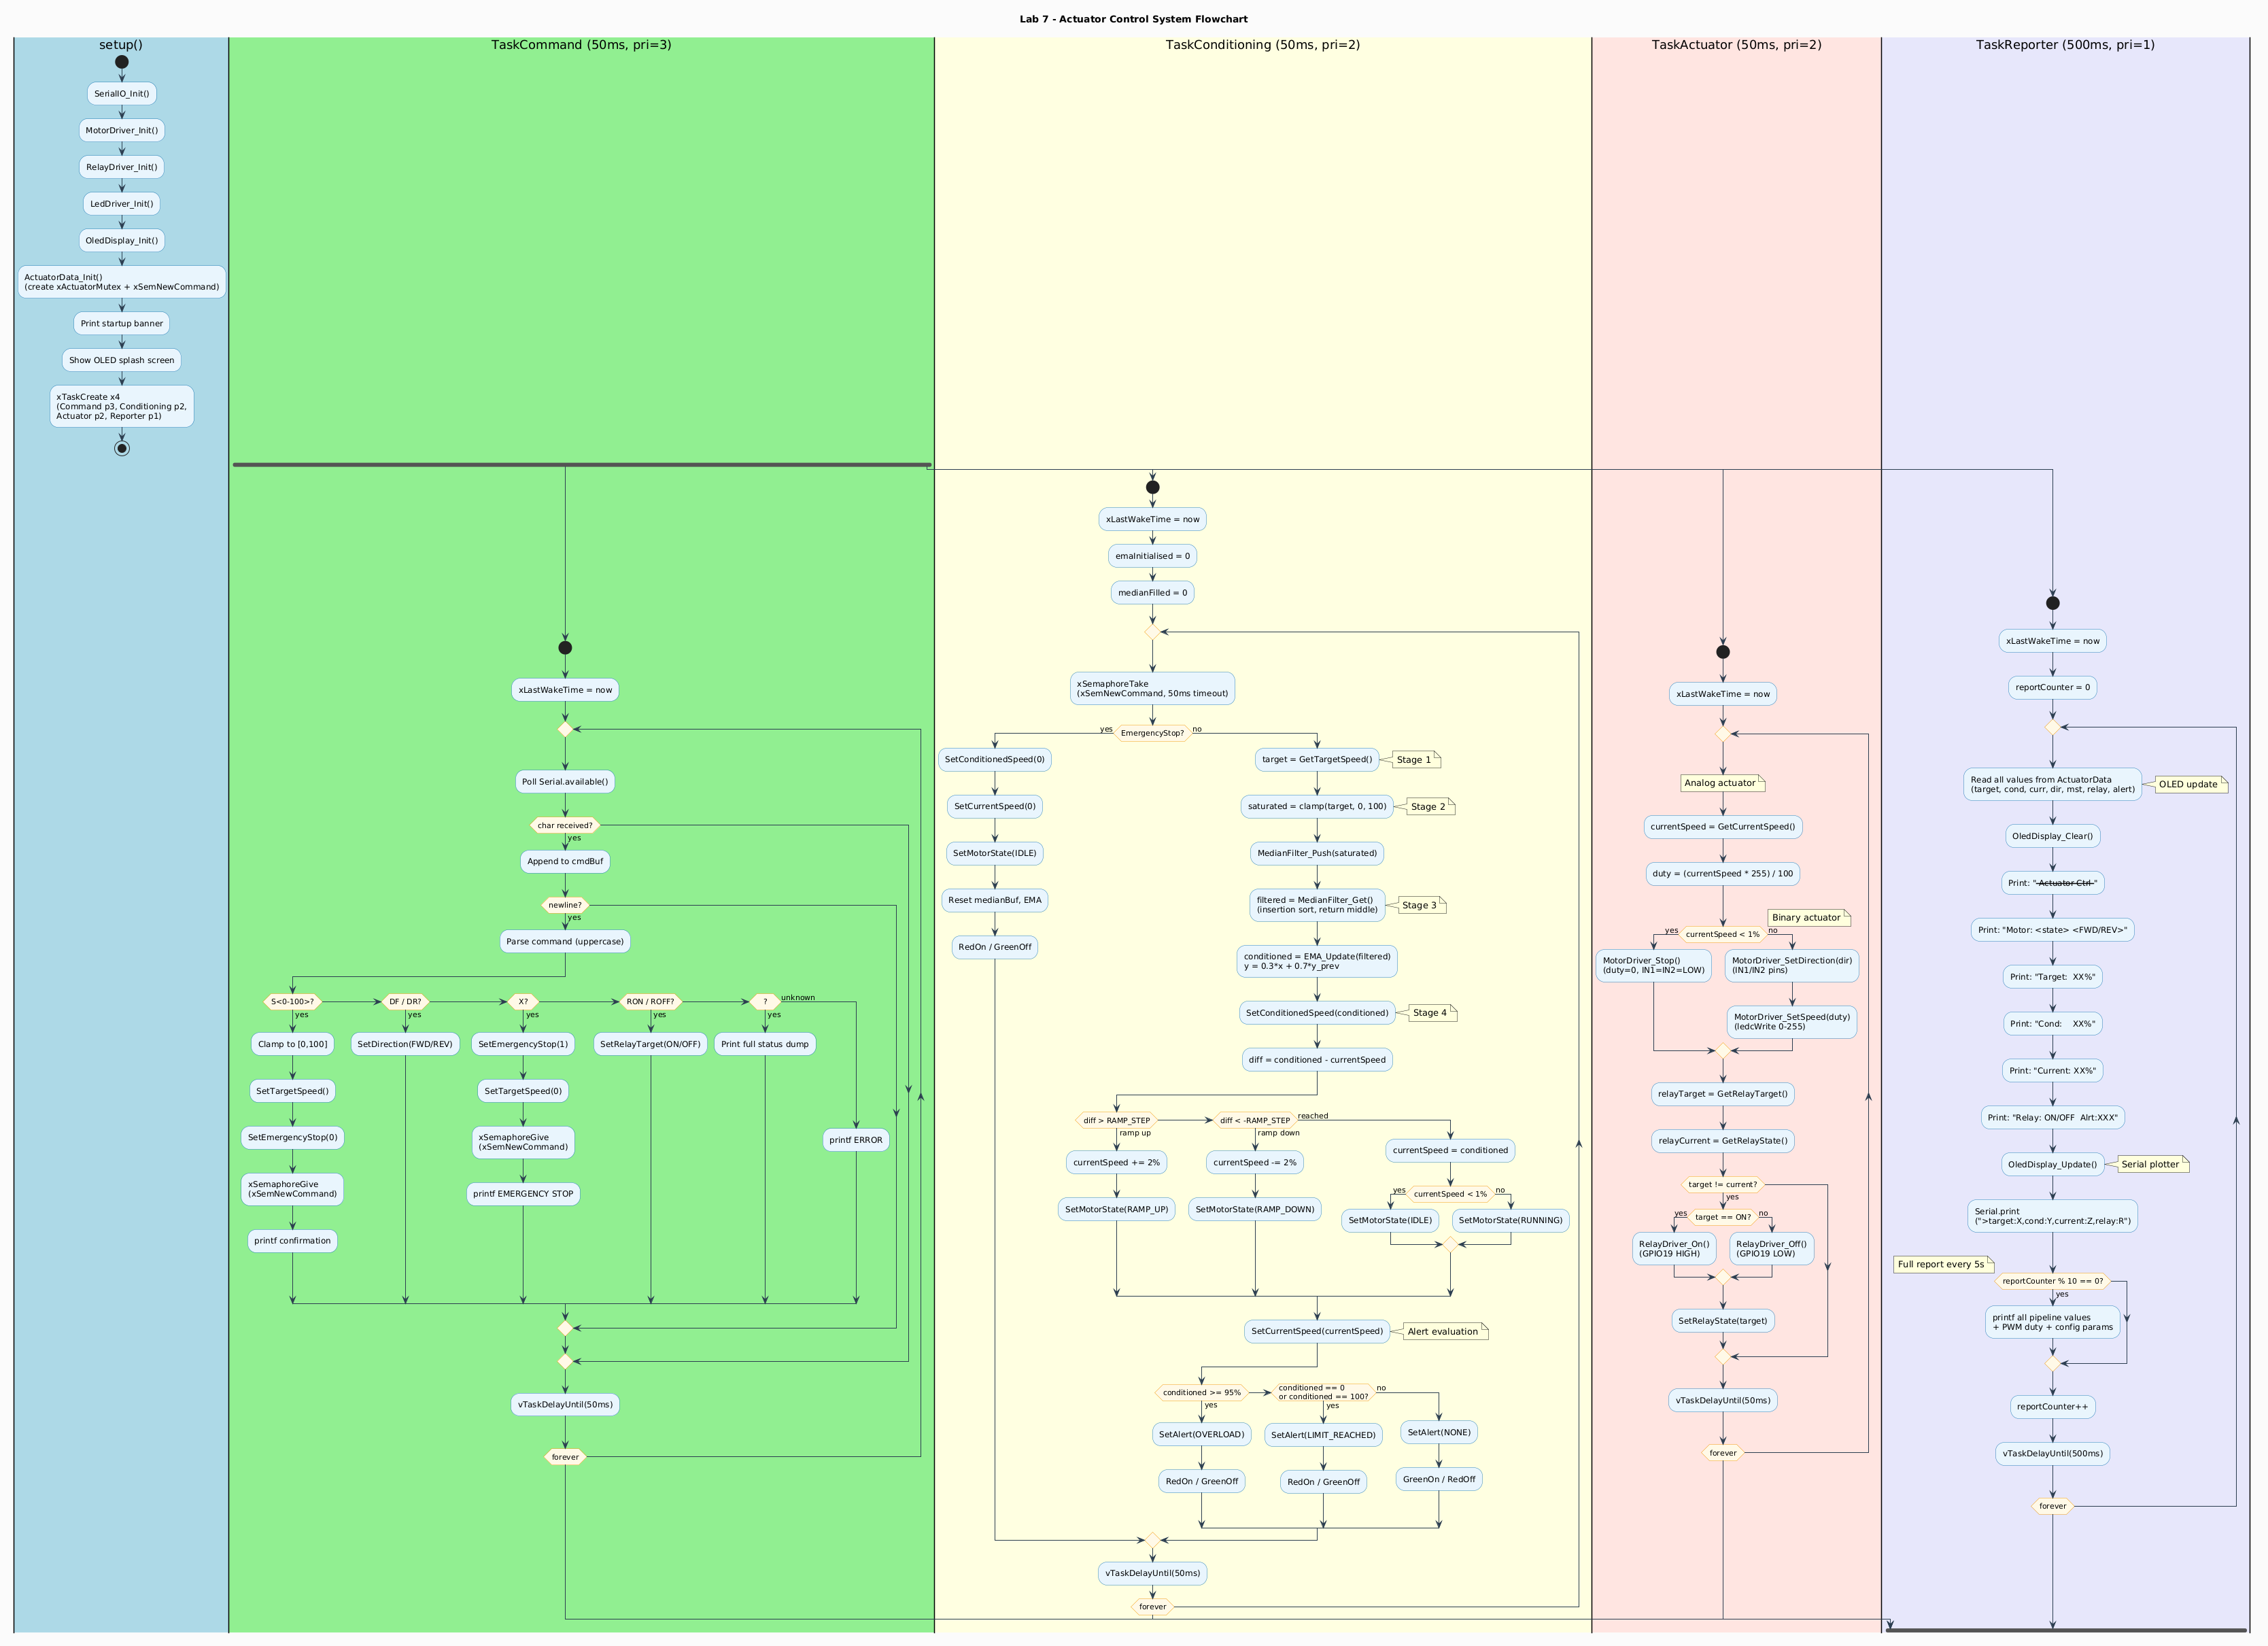
\includegraphics[width=1\textwidth]{./img/flow.png}
    \caption{Flow chart of the algorithm}
    \label{fig:flow}
\end{figure}

\clearpage
\subsection{Code design}

Code is developed following the principle of separating the interface from the
implementation, by creating for each header file \texttt{.h} a respective \texttt{.cpp}
file. The project uses \textbf{PlatformIO} with three library directories:

\begin{enumerate}
  \item \textbf{MCAL layer} (\texttt{lib/MCAL/GpioDriver}) -- hardware-specific code
    that wraps \texttt{Arduino.h} GPIO calls. All direct hardware access is encapsulated
    here.
  \item \textbf{ECAL layer} (\texttt{lib/ECAL/}) -- electronic component drivers:
    \texttt{MotorDriver} (L298N PWM via LEDC + direction pins, GPIO~16/17/18),
    \texttt{RelayDriver} (GPIO~19 on/off),
    \texttt{LedDriver} (two status LEDs, GPIO~25/26),
    \texttt{OledDisplay} (Adafruit SSD1306 128$\times$64), and
    \texttt{SerialIO} (UART initialization).
    Each driver header declares its connection pins for easy circuit reference.
  \item \textbf{SRV layer} (\texttt{lib/SRV/}) -- the \texttt{ActuatorData} shared-state
    module and the four FreeRTOS task implementations.
\end{enumerate}

The \texttt{MotorDriver} initializes the LEDC peripheral and provides a clean API that
is identical for a real motor or an LED:

\begin{lstlisting}
void MotorDriver_Init(void)
{
    GpioDriver_PinMode(MOTOR_IN1_PIN, OUTPUT);
    GpioDriver_PinMode(MOTOR_IN2_PIN, OUTPUT);
    GpioDriver_Write(MOTOR_IN1_PIN, LOW);
    GpioDriver_Write(MOTOR_IN2_PIN, LOW);
    ledcSetup(MOTOR_LEDC_CHANNEL, MOTOR_LEDC_FREQ, MOTOR_LEDC_RES);
    ledcAttachPin(MOTOR_ENA_PIN, MOTOR_LEDC_CHANNEL);
    ledcWrite(MOTOR_LEDC_CHANNEL, 0);
}

void MotorDriver_SetSpeed(uint8_t duty)   // 0-255
{
    currentDuty = duty;
    ledcWrite(MOTOR_LEDC_CHANNEL, duty);
}

void MotorDriver_SetDirection(uint8_t dir) // 0=forward, 1=reverse
{
    if (dir == 0) {
        GpioDriver_Write(MOTOR_IN1_PIN, HIGH);
        GpioDriver_Write(MOTOR_IN2_PIN, LOW);
    } else {
        GpioDriver_Write(MOTOR_IN1_PIN, LOW);
        GpioDriver_Write(MOTOR_IN2_PIN, HIGH);
    }
}
\end{lstlisting}

The \texttt{ActuatorData} module centralizes all shared data behind mutex-protected
getters and setters, and owns the FreeRTOS synchronization primitives:

\begin{lstlisting}
// Declared in ActuatorData.h, initialized in ActuatorData_Init()
extern SemaphoreHandle_t xSemNewCommand;  // binary semaphore: new speed command
extern SemaphoreHandle_t xActuatorMutex; // mutex: protects all shared actuator fields
\end{lstlisting}

The signal conditioning pipeline in \texttt{TaskConditioning} applies all four stages
then manages motor state transitions:
\begin{lstlisting}
/* 1. Saturation */
float saturated = Saturate(target);  // clamp to [0, 100]

/* 2. Median filter (window=5) */
MedianFilter_Push(saturated);
float filtered = MedianFilter_Get();

/* 3. EMA smoothing (alpha=0.3) */
float conditioned = EMA_Update(filtered);
ActuatorData_SetConditionedSpeed(conditioned);

/* 4. Ramping (2% per cycle) */
float diff = conditioned - currentSpeed;
if      (diff >  RAMP_STEP) { currentSpeed += RAMP_STEP; state = MOTOR_RAMP_UP;   }
else if (diff < -RAMP_STEP) { currentSpeed -= RAMP_STEP; state = MOTOR_RAMP_DOWN; }
else    { currentSpeed = conditioned;
          state = (currentSpeed < 1.0f) ? MOTOR_IDLE : MOTOR_RUNNING; }
ActuatorData_SetCurrentSpeed(currentSpeed);
\end{lstlisting}

TaskActuator maps the conditioned speed to a PWM duty cycle and applies it:
\begin{lstlisting}
float currentSpeed = ActuatorData_GetCurrentSpeed();
uint8_t duty = (uint8_t)((currentSpeed * 255.0f) / 100.0f);

if (currentSpeed < 1.0f) {
    MotorDriver_Stop();
} else {
    MotorDriver_SetDirection((uint8_t)dir);
    MotorDriver_SetSpeed(duty);
}
\end{lstlisting}

TaskReporter uses \texttt{vTaskDelayUntil} for drift-corrected 500\,ms periodicity
and outputs data in the \texttt{>name:value} format compatible with the VS Code
Serial Plotter extension:
\begin{lstlisting}
// Serial Plotter line (every 500 ms)
Serial.print(">");
Serial.print("target:"); Serial.print(target);
Serial.print(",cond:");   Serial.print(cond, 1);
Serial.print(",current:"); Serial.print(curr, 1);
Serial.print(",relay:");  Serial.print(relay == RELAY_ON ? 1 : 0);
Serial.println();

// Full structured report (every 5 s)
if ((reportCounter++ % FULL_REPORT_EVERY) == 0) {
    printf("Target speed  : %d%%\n", target);
    printf("Conditioned   : %.1f%%  (median=%d, EMA alpha=%.2f)\n",
           cond, MEDIAN_WINDOW, EMA_ALPHA);
    printf("Current speed : %.1f%%  (ramp step=%d/cyc)\n", curr, RAMP_STEP);
    printf("Motor state   : %s\n", MotorStateName(mst));
    printf("Relay         : %s\n", relay == RELAY_ON ? "ON" : "OFF");
    printf("Alert         : %s\n", AlertName(alert));
\end{lstlisting}
